\documentclass[14pt,compress,t,noamsthm,notheorem,table,handout,fontset=none]{ctexbeamer}

\setCJKmainfont[
  Path=/usr/local/texlive/2024/texmf-dist/fonts/opentype/public/fandol/,
  BoldFont=FandolSong-Bold.otf
]{FandolSong-Regular.otf}
\setCJKsansfont[
  Path=/usr/local/texlive/2024/texmf-dist/fonts/opentype/public/fandol/,
  BoldFont=FandolHei-Bold.otf
]{FandolHei-Regular.otf}
\setCJKmonofont[
  Path=/usr/local/texlive/2024/texmf-dist/fonts/opentype/public/fandol/
]{FandolFang-Regular.otf}
\setsansfont[
  Path=/usr/local/texlive/2024/texmf-dist/fonts/opentype/public/tex-gyre/,
  BoldFont=texgyreheros-bold.otf,
  ItalicFont=texgyreheros-italic.otf,
  BoldItalicFont=texgyreheros-bolditalic.otf
]{texgyreheros-regular.otf}
\setmonofont[
  Path=/usr/local/texlive/2024/texmf-dist/fonts/opentype/public/inconsolata/,
  BoldFont=Inconsolatazi4-Bold.otf,
  StylisticSet=3
]{Inconsolatazi4-Regular.otf}
\usetheme{default}
\usefonttheme[onlymath]{serif}
\setbeamertemplate{navigation symbols}{}
\usepackage{amsmath,amssymb}
\usepackage{booktabs}
\usepackage{graphicx}
\usepackage{hyperref}
\usepackage{listings}
\usepackage{xcolor}
\usepackage{etoolbox}
\graphicspath{{figs/}}
\definecolor{navy}{HTML}{193B5B}
\definecolor{bodytext}{HTML}{24313D}
\definecolor{muted}{HTML}{617080}
\definecolor{rulegray}{HTML}{CBD4DD}
\definecolor{codebg}{HTML}{F4F6F8}
\definecolor{codeframe}{HTML}{D5DDE5}
\definecolor{codecomment}{HTML}{4B705C}
\definecolor{codestring}{HTML}{92533C}
\definecolor{tablehead}{HTML}{EEF2F6}
\hypersetup{pdfborder=0 0 0,colorlinks=true,linkcolor=navy,urlcolor=navy}
\setbeamercolor{normal text}{fg=bodytext,bg=white}
\setbeamercolor{structure}{fg=navy}
\setbeamercolor{frametitle}{fg=navy,bg=white}
\setbeamercolor{myfootline}{bg=white,fg=muted}
\setbeamercolor{block title}{fg=navy,bg=white}
\setbeamercolor{block body}{fg=bodytext,bg=white}
\setbeamercolor{alerted text}{fg=codestring}
\setbeamerfont{frametitle}{size=\fontsize{18}{21},series=\bfseries}
\setbeamerfont{block title}{size=\normalsize,series=\bfseries}
\setbeamertemplate{blocks}[default]
\setbeamertemplate{itemize item}{\raisebox{0.15ex}{\scriptsize\textbullet}}
\setbeamertemplate{enumerate item}{\insertenumlabel.}
\AtBeginEnvironment{itemize}{\setlength{\itemsep}{0.24em}}
\AtBeginEnvironment{enumerate}{\setlength{\itemsep}{0.24em}}
\arrayrulecolor{rulegray}
\setlength{\heavyrulewidth}{0.6pt}
\setlength{\lightrulewidth}{0.35pt}
\setbeamertemplate{headline}{}
\setbeamertemplate{footline}{%
  \leavevmode\mbox{%
    \begin{beamercolorbox}[wd=.75\paperwidth,ht=3mm,dp=2mm,left]{myfootline}%
      \hspace*{0.8cm}{\fontsize{7.5}{9}\selectfont 统计学导论上机课}
    \end{beamercolorbox}%
    \begin{beamercolorbox}[wd=.25\paperwidth,ht=3mm,dp=2mm,right]{myfootline}%
      {\fontsize{7.5}{9}\selectfont\insertframenumber\,/\,\inserttotalframenumber\hspace*{0.8cm}}
    \end{beamercolorbox}}
  \vskip0pt}
\setbeamertemplate{frametitle}{%
  \vspace{0.28cm}%
  {\usebeamerfont{frametitle}\usebeamercolor[fg]{frametitle}\insertframetitle\par}%
  \vspace{0.12cm}%
  {\color{rulegray}\hrule height 0.45pt}%
  \vspace{-0.2cm}}
\setbeamersize{text margin left=0.8cm,text margin right=0.8cm}
\setbeamertemplate{title page}{%
  \vspace*{0.95cm}%
  {\fontsize{25}{31}\selectfont\bfseries\color{navy}\inserttitle\par}%
  \vspace{0.35cm}%
  {\fontsize{14}{19}\selectfont\color{bodytext}\insertsubtitle\par}%
  \vspace{0.65cm}%
  {\color{rulegray}\hrule height 0.45pt}%
  \vspace{0.6cm}%
  {\fontsize{13}{18}\selectfont\insertauthor\par}%
  \vspace{0.12cm}%
  {\fontsize{10}{15}\selectfont\color{muted}\insertinstitute\par}%
  \vfill
  {\fontsize{10}{14}\selectfont\color{muted}\insertdate\par}%
  \vspace*{0.6cm}}
\lstset{
  language=R,
  basicstyle=\ttfamily\fontsize{12.5}{14.5}\selectfont\color{bodytext},
  keywordstyle=\color{navy},
  commentstyle=\color{codecomment},
  stringstyle=\color{codestring},
  backgroundcolor=\color{codebg},
  frame=single,
  rulecolor=\color{codeframe},
  framerule=0.35pt,
  framesep=5pt,
  showstringspaces=false,
  keepspaces=true,
  breaklines=true,
  columns=fullflexible,
  xleftmargin=5pt,
  xrightmargin=5pt,
  aboveskip=0.35em,
  belowskip=0.35em
}
\lstdefinestyle{output}{
  language={},
  keywordstyle=\color{bodytext},
  commentstyle=\color{bodytext},
  stringstyle=\color{bodytext},
  backgroundcolor=\color{white},
  frame=none,
  aboveskip=0.12em,
  belowskip=0.25em
}
\newcommand{\code}[1]{\textcolor{navy}{\texttt{#1}}}
\newcommand{\inputlabel}{\par\smallskip{\fontsize{10.5}{13}\selectfont\bfseries\color{muted}输入代码\par}}
\newcommand{\outputlabel}{\par\smallskip{\fontsize{10.5}{13}\selectfont\bfseries\color{muted}Console 输出\par}}
\newcommand{\thead}[1]{\textcolor{navy}{\textbf{#1}}}

\title{R语言基础（五）}
\subtitle{随机模拟与正态近似}
\author{郑泽靖}
\institute{北京师范大学统计学院}
\date{2026年秋季学期}

\begin{document}

% 第一节45分钟：回顾2，随机数5，大数定律及应用8，MC积分5，正态概率10，练习10，讲评5。
% 第二节45分钟：回顾3，CLT7，体重例8，泊松模拟12，练习10，讲评5。

\begin{frame}[plain]
  \titlepage
  \note{教材第84--93页。封面不另计时。本讲两节，各45分钟。第一节随机模拟与蒙特卡罗方法，第二节中心极限定理及应用。各保留10分钟课堂练习和5分钟讲评，无需提交作业。}
\end{frame}

\begin{frame}[fragile]{回顾：平均值与频率}
  \inputlabel
\begin{lstlisting}
x <- c(0, 1, 1, 0, 1)
mean(x)
mean(x == 1)
\end{lstlisting}
  \outputlabel
\begin{lstlisting}[style=output]
[1] 0.6
[1] 0.6
\end{lstlisting}
  \code{mean(x)} 计算平均值。\par\smallskip
  对逻辑值求平均时，\par
  \code{TRUE} 按1计算，\code{FALSE} 按0计算。\par
  因此可得到条件成立的频率。
  \note{教材第85--86页，衔接R-3的mean与逻辑频率。第一节回顾2分钟。教师演示并请学生解释0.6。}
\end{frame}

\begin{frame}[fragile]{均匀分布随机数：runif()}
  生成区间 $(0,1)$ 上均匀分布的随机数。
  \inputlabel
\begin{lstlisting}
x <- runif(10, 0, 1)
x
mean(x)
\end{lstlisting}
  \begin{itemize}
    \item 第一个参数10是生成的个数。
    \item 后两个参数0、1是区间端点。
    \item 重复运行通常会得到不同结果。
  \end{itemize}
  \note{教材第84页案例2.17、第88页runif程序。第一节随机数5分钟中的3分钟，学生跟随运行。只解释本例参数，不扩展随机数原理。}
\end{frame}

\begin{frame}[fragile]{正态分布随机数：rnorm()}
  生成标准正态分布 $N(0,1)$ 的随机数。
  \inputlabel
\begin{lstlisting}
x <- rnorm(10, 0, 1)
x
\end{lstlisting}
  \begin{itemize}
    \item 10是生成的个数，0是均值，1是标准差。
    \item 标准正态随机数可以取正值，也可以取负值。
  \end{itemize}
  \note{教材第89页正态随机数程序。第一节随机数5分钟中的2分钟，教师演示。学生仅掌握本例三个参数的含义。}
\end{frame}

\begin{frame}{大数定律}
  设 $X_1,\ldots,X_n$ 是 $X$ 的独立、同分布重复观测，\\
  且 $X$ 的数学期望为有限数。
  \[
    \lim_{n\to\infty}\frac{1}{n}\sum_{k=1}^n X_k
    =\mathrm{E}(X)
  \]
  上述等式成立的概率为1。\par\medskip
  可以用大量重复观测的平均值估计数学期望。\par\smallskip
  本讲通过计算与图形理解结论，不讨论证明。
  \note{教材第85页定理2.6.1，保留重复观测和有限期望条件。第一节大数定律及应用8分钟中的2分钟。说明“概率为1”的结论不等于每次有限次计算都相同。}
\end{frame}

\begin{frame}[fragile]{均匀分布的样本平均值}
  对 $X\sim U(0,1)$，有 $\mathrm{E}(X)=0.5$。
  \inputlabel
\begin{lstlisting}
x <- runif(50000, 0, 1)
mean(x[1:100])
mean(x[1:1000])
mean(x)
\end{lstlisting}
  三次平均分别使用100、1000、50000个观测。\par\smallskip
  大样本下平均值通常更接近0.5，\par
  但误差不必逐次减小。
  \note{教材第84页案例2.17。第一节大数定律及应用8分钟中的1分钟，教师演示同一组数据不同前缀的平均值。}
\end{frame}

\begin{frame}{平均值随观测次数的变化}
  \centering
  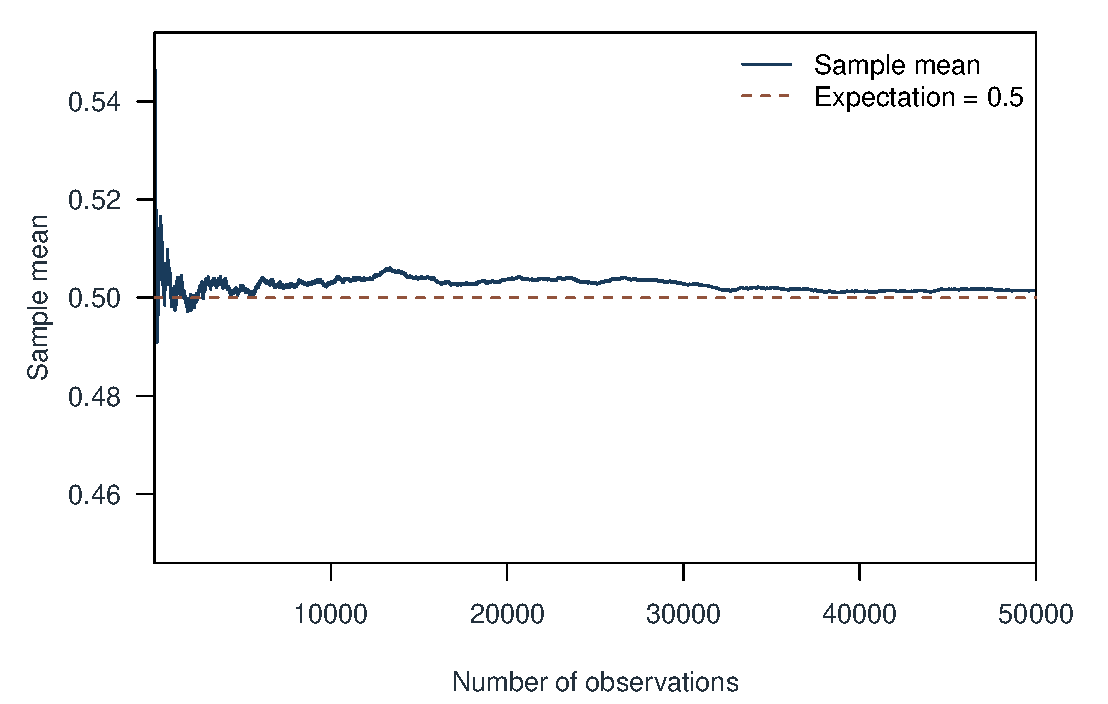
\includegraphics[width=0.94\linewidth,height=5.8cm,keepaspectratio]{uniform-mean.pdf}
  \par\smallskip
  \raggedright\small 图形对应一次模拟。曲线会波动，不必单调接近0.5。
  \note{教材第84页图2.19。图由R生成，50000次U(0,1)重复观测的前缀平均值，虚线为期望0.5。第一节大数定律及应用8分钟中的1分钟，教师引导读图，不要求学生独立编写作图程序。}
\end{frame}

\begin{frame}[fragile]{矩的平均与频率}
  \small
  例2.6.1：若 $\mathrm{E}(X^k)$ 有限，可用 $X_i^k$ 的平均估计它。
  \inputlabel
\begin{lstlisting}
x <- runif(10000, 0, 1)
mean(x^2)
mean(x <= 0.5)
\end{lstlisting}
  \begin{itemize}
    \item 第一项估计 $\mathrm{E}(X^2)$。
    \item 第二项计算 $X\leq0.5$ 的频率，估计其概率。
  \end{itemize}
  例2.6.2的含义：频率是0、1取值的平均，能用于估计概率。
  \note{教材第85--86页例2.6.1和2.6.2。第一节大数定律及应用8分钟中的2分钟。只解释已有幂运算和mean的组合，不推导均匀分布二阶矩。}
\end{frame}

\begin{frame}[fragile]{经验分布函数}
  对给定的 $t$，经验分布函数表示\\
  观测值中不大于 $t$ 的比例。
  \[
    F_n(t)=\frac{\text{不大于 }t\text{ 的观测个数}}{n}
    \ \approx\ F(t)=\mathrm{P}(X\leq t).
  \]
  \inputlabel
\begin{lstlisting}
x <- runif(10000, 0, 1)
t <- 0.5
mean(x <= t)
\end{lstlisting}
  例2.6.3：对给定的 $t$，可用 $F_n(t)$ 估计 $F(t)$。
  \note{教材第86--87页定义2.6.1、例2.6.3。第一节大数定律及应用8分钟中的2分钟，解释“累计比例”。保持教材范围，不引入ecdf函数或一致收敛。}
\end{frame}

\begin{frame}{蒙特卡罗积分}
  蒙特卡罗方法：用随机模拟解决计算问题。\par\medskip
  例2.6.4：设 $f$ 在 $[a,b]$ 上连续，取 $U\sim U(a,b)$。
  \[
    \int_a^b f(x)\,\mathrm{d}x
    =(b-a)\mathrm{E}\{f(U)\}.
  \]
  用 $n$ 个均匀分布随机数 $U_1,\ldots,U_n$，得到
  \[
    \int_a^b f(x)\,\mathrm{d}x
    \approx (b-a)\frac{1}{n}\sum_{k=1}^n f(U_k).
  \]
  \note{教材第87页例2.6.4与蒙特卡罗方法定义。第一节MC积分5分钟中的3分钟。只说明“区间长度乘函数值平均”，不作积分理论推导。}
\end{frame}

\begin{frame}{积分近似的计算步骤}
  \begin{enumerate}
    \item 在积分区间 $[a,b]$ 中生成均匀随机数。
    \item 计算每个随机数对应的函数值 $f(U_k)$。
    \item 计算函数值的平均，再乘区间长度 $b-a$。
  \end{enumerate}
  \medskip
  每次运行所用的随机数不同，近似值通常也不同。\par\smallskip
  增大模拟次数有助于提高精度，但一次结果不保证更接近目标值。
  \note{教材第87页公式2.72及第88页思考题。第一节MC积分5分钟中的2分钟，联系下一页例2.6.5。}
\end{frame}

\begin{frame}{教材例2.6.5：标准正态区间概率}
  设 $X\sim N(0,1)$，计算 $\mathrm{P}(0.1<X<2)$。\par\medskip
  标准正态密度为
  \[
    \varphi(x)=\frac{1}{\sqrt{2\pi}}\exp\left(-\frac{x^2}{2}\right).
  \]
  因此
  \[
    \mathrm{P}(0.1<X<2)=\int_{0.1}^{2}\varphi(x)\,\mathrm{d}x.
  \]
  可以用均匀随机数近似计算这个积分。
  \note{教材第88页例2.6.5。第一节正态概率10分钟中的2分钟，教师说明计算对象与正态密度。}
\end{frame}

\begin{frame}[fragile]{方法一：均匀随机数计算积分}
  \inputlabel
\begin{lstlisting}
Y <- runif(10000, 0.1, 2)
c <- 1 / sqrt(2 * pi)
f <- c * exp(-(Y * Y) / 2)
p <- (2 - 0.1) * mean(f)
p
\end{lstlisting}
  \begin{itemize}
    \item \code{sqrt()} 计算平方根，\code{exp()} 计算指数函数。
    \item \code{pi} 是 R 中的圆周率常量。
    \item \code{f} 保存密度值，\code{p} 保存近似概率。
  \end{itemize}
  \note{教材第88页例2.6.5原程序，排版规范化并显式显示p。第一节正态概率10分钟中的3分钟，教师逐行演示，学生运行课堂程序相应段。}
\end{frame}

\begin{frame}[fragile]{方法二：正态随机数计算频率}
  直接生成标准正态随机数，计算落入区间的比例。
  \inputlabel
\begin{lstlisting}
x <- rnorm(100000, 0, 1)
I <- x > 0.1 & x < 2
p <- mean(I)
p
\end{lstlisting}
  \code{I} 保存每个随机数是否落在 $(0.1,2)$ 中。\par\smallskip
  \code{mean(I)} 是条件成立的频率，近似所求概率。
  \note{教材第89页例2.6.5第二种方法。第一节正态概率10分钟中的3分钟。复用R-3已学的逻辑运算及mean，不引入其他模拟方法。}
\end{frame}

\begin{frame}[fragile]{用 pnorm() 核对}
  \code{pnorm(t, 0, 1)} 给出标准正态概率 $\mathrm{P}(X\leq t)$。
  \inputlabel
\begin{lstlisting}
pnorm(2, 0, 1) - pnorm(0.1, 0, 1)
\end{lstlisting}
  \outputlabel
\begin{lstlisting}[style=output]
[1] 0.437422
\end{lstlisting}
  两种模拟方法都在估计约0.4374的同一个概率。\par\smallskip
  模拟值与计算值有差异，不需要与本页完全相同。
  \note{教材第88--89页pnorm校核。第一节正态概率10分钟中的2分钟。连续分布端点概率为0，不在此另加端点知识讲解。}
\end{frame}

\begin{frame}{课堂练习一：重复模拟}
  \begin{enumerate}
    \item 运行例2.6.5的两段模拟程序，各重复两次，记录近似概率。
    \item 方法一把10000改为100000，再运行一次。
    \item 方法二把100000改为10000，再运行一次。
    \item 与0.437422比较，\\
      用一句话说明运行结果的差异。
  \end{enumerate}
  \medskip
  使用 \code{R5-class.R} 第5、6段的完整程序。\par\smallskip
  课堂完成，无需提交。
  \note{教材第88--89页例2.6.5及思考题。第一节独立练习10分钟。学生只修改模拟次数，不要求封装函数、编写循环或计算误差阶。}
\end{frame}

\begin{frame}[fragile]{练习一参考：两种计算程序}
  \small
  均匀随机数与密度值平均：
\begin{lstlisting}
Y <- runif(100000, 0.1, 2)
f <- exp(-(Y * Y) / 2) / sqrt(2 * pi)
(2 - 0.1) * mean(f)
\end{lstlisting}
  正态随机数与区间频率：
\begin{lstlisting}
x <- rnorm(10000, 0, 1)
mean(x > 0.1 & x < 2)
\end{lstlisting}
  两段程序的结果都应接近0.4374。
  \note{教材第88--89页例2.6.5。第一节讲评5分钟中的3分钟。核对区间条件、区间长度因子及mean的对象，不给随机输出的固定标准答案。}
\end{frame}

\begin{frame}{第一节小结}
  \begin{itemize}
    \item 随机数模拟重复观测，每次结果通常不同。
    \item 观测平均值可估计数学期望，\par
          观测频率可估计概率。
    \item 蒙特卡罗积分使用函数值平均与区间长度。
    \item 模拟次数增加时，误差仍可能局部增大。
  \end{itemize}
  \medskip
  例2.6.5的两种方法，都在计算\par
  同一个正态区间概率。
  \note{教材第84--89页。第一节讲评5分钟中的2分钟。第一节累计45分钟，收束后课间休息。}
\end{frame}

\begin{frame}{第二节：样本平均值的分布}
  上一节用样本平均值估计数学期望。
  \[
    \overline{X}_n=\frac{1}{n}\sum_{k=1}^n X_k.
  \]
  若重新抽取一组样本，$\overline{X}_n$ 也会改变。\par\medskip
  本节研究标准化后的样本平均值\par
  如何用正态分布近似。
  \note{教材第89--90页中心极限定理的引入。第二节回顾3分钟。区别一组样本中的n个观测与重复抽取多组样本，不讲估计误差阶。}
\end{frame}

\begin{frame}{样本平均值的标准化}
  记 $\mu=\mathrm{E}(X)$、$\sigma^2=\mathrm{D}(X)>0$。
  \[
    Z_n=\frac{\sqrt{n}(\overline{X}_n-\mu)}{\sigma}
       =\frac{\overline{X}_n-\mu}{\sigma/\sqrt{n}}.
  \]
  \begin{itemize}
    \item 减去 $\mu$，使中心位于0。
    \item 除以 $\sigma/\sqrt{n}$，使标准差为1。
  \end{itemize}
  标准化后可与标准正态分布比较。
  \note{教材第90页公式2.73。第二节CLT7分钟中的3分钟。只说明均值和标准差的作用，公式的推导不计入上机课。}
\end{frame}

\begin{frame}{中心极限定理}
  设 $X_1,\ldots,X_n$ 是 $X$ 的独立、同分布重复观测，且
  \[
    0<\sigma^2=\mathrm{D}(X)<\infty.
  \]
  对任意实数 $t$，有
  \[
    \lim_{n\to\infty}\mathrm{P}(Z_n\leq t)=\Phi(t).
  \]
  $\Phi$ 是标准正态分布函数。\par\smallskip
  当 $n$ 较大时，用 $N(0,1)$ 近似 $Z_n$ 的分布。
  \note{教材第91页定理2.6.2。第二节CLT7分钟中的2分钟。保留有限且正的方差条件，不证明定理，不宣称任意有限n均准确。}
\end{frame}

\begin{frame}{大数定律与中心极限定理}
  \small
  \renewcommand{\arraystretch}{1.4}
  \begin{tabular*}{\linewidth}{@{\extracolsep{\fill}}p{0.26\linewidth}p{0.65\linewidth}@{}}
    \toprule
    \thead{结论} & \thead{本讲中的用途} \\
    \midrule
    大数定律 & 用样本平均值估计数学期望，\newline 用频率估计概率。 \\
    中心极限定理 & 用标准正态分布近似\newline 标准化样本平均值的分布。 \\
    \bottomrule
  \end{tabular*}
  \par\medskip
  后者不要求原变量 $X$ 本身服从正态分布，\par
  但需要定理中的重复观测与方差条件。
  \note{教材第89--92页。第二节CLT7分钟中的2分钟。教材案例2.18的图形比较旨在理解正态近似，本讲随后以例2.6.7的模拟呈现同一含义，不增加二项图绘图任务。}
\end{frame}

\begin{frame}{教材例2.6.6：平均体重的概率}
  已知某大学女学生体重的均值为51.96 kg，\\
  标准差为6.31 kg。\par\medskip
  随机选择36名女大学生，\\
  求平均体重超过57 kg的概率。\par\medskip
  记36人的平均体重为 $\overline X$，用中心极限定理近似：
  \[
    \mathrm{P}(\overline X>57)
    \approx 1-\Phi\left(\frac{\sqrt{36}(57-51.96)}{6.31}\right).
  \]
  \note{教材第92页例2.6.6。第二节体重例8分钟中的3分钟。教师确认单位、样本量和“平均超过57”的事件，不改教材数值。}
\end{frame}

\begin{frame}[fragile]{例2.6.6的 R 计算}
  \inputlabel
\begin{lstlisting}
z <- sqrt(36) * (57 - 51.96) / 6.31
z
1 - pnorm(z, 0, 1)
\end{lstlisting}
  \outputlabel
\begin{lstlisting}[style=output]
[1] 4.792393
[1] 8.240182e-07
\end{lstlisting}
  \code{e-07} 表示乘以 $10^{-7}$。\par\smallskip
  按教材的正态近似，所求概率很小。
  \note{教材第92页例2.6.6程序与结果。第二节体重例8分钟中的3分钟，学生跟随运行。1-pnorm写法与教材一致，不添加数值稳定性话题。}
\end{frame}

\begin{frame}{例2.6.6的结果解释}
  \begin{itemize}
    \item 计算对象是36人平均体重超过57 kg的概率。
    \item 标准化时使用平均值的标准差 $6.31/\sqrt{36}$。
    \item 结果是中心极限定理给出的近似值。
  \end{itemize}
  \medskip
  教材没有假设单个人的体重一定服从正态分布。\par\smallskip
  正态近似仍需满足重复观测等定理条件。
  \note{教材第92页例2.6.6后说明。第二节体重例8分钟中的2分钟。强调平均值与单个观测的区别，不增加新的例题。}
\end{frame}

\begin{frame}{教材例2.6.7：泊松样本的标准化均值}
  设 $X\sim\mathrm{P}(0.5)$，其均值、方差都为0.5。\par\medskip
  每组取 $n=30$ 个重复观测，计算
  \[
    \overline X=\frac{1}{30}\sum_{k=1}^{30}X_k,
    \qquad Z=\frac{\sqrt{30}(\overline X-0.5)}{\sqrt{0.5}}.
  \]
  重复生成1000组样本，得到1000个 $Z$ 值。\par\smallskip
  将它们的经验分布函数与 $\Phi$ 比较。
  \note{教材第92页例2.6.7。第二节泊松模拟12分钟中的2分钟。教师演示，学生使用给定完整程序，不从零编写长程序。泊松均值与方差采用教材已知结论，不推导。}
\end{frame}

\begin{frame}[fragile]{生成1000组泊松样本}
  \inputlabel
\begin{lstlisting}
n <- 30
y <- matrix(rpois(1000 * n, 0.5),
            1000, n)
z <- (rowSums(y) / n - 0.5) *
     sqrt(n / 0.5)
\end{lstlisting}
  \begin{itemize}
    \item \code{rpois()} 生成泊松分布随机数，参数0.5。
    \item \code{y} 有1000行、$n$ 列，每行是一组样本。
    \item \code{rowSums(y) / n} 是每组的样本平均值。
  \end{itemize}
  \note{教材第92页例2.6.7，参数化n以便教材第93页练习。第二节泊松模拟12分钟中的3分钟，教师结合矩阵行列解释，仅引入本例rpois参数。}
\end{frame}

\begin{frame}[fragile]{计算标准化均值的经验累计比例}
  \inputlabel
\begin{lstlisting}
x <- seq(-3, 3, 0.1)
f <- c()
for (i in 1:length(x)) {
  f <- c(f, sum(z <= x[i]) / 1000)
}
phi <- pnorm(x, 0, 1)
\end{lstlisting}
  \code{f} 保存各位置的经验累计比例。\par\smallskip
  \code{phi} 保存相同位置的标准正态累计概率。
  \note{教材第92页例2.6.7。第二节泊松模拟12分钟中的3分钟。解释length(x)是x中元素个数，for/c/sum均为前讲内容。与教材一致采用小于等于；不引入ecdf或其他函数。}
\end{frame}

\begin{frame}[fragile]{经验分布与标准正态分布的比较}
  \small
  \code{R5-class.R} 已提供完整绘图段。核心代码为：
\begin{lstlisting}
plot(x, phi, type = "l", ylim = c(0, 1))
for (i in 1:(length(x) - 1)) {
  lines(x[i:(i + 1)], c(f[i], f[i]),
        col = "red")
  points(x[i], f[i], pch = 20,
         col = "red")
}
\end{lstlisting}
  黑线表示 $\Phi$，红色线段与点表示经验累计比例。\par\smallskip
  本例重点是比较曲线，绘图参数不要求独立编写。
  \note{教材第93页绘图段，修正plot中对象名为已计算的phi，避免教材排印不一致。简化为在每个网格位置画点，仍沿用plot/lines/points，完整程序含标签及图例。第二节泊松模拟12分钟中的1分钟，教师运行现成代码，不逐项讲解作图参数。}
\end{frame}

\begin{frame}{30个观测的样本：一次模拟结果}
  \centering
  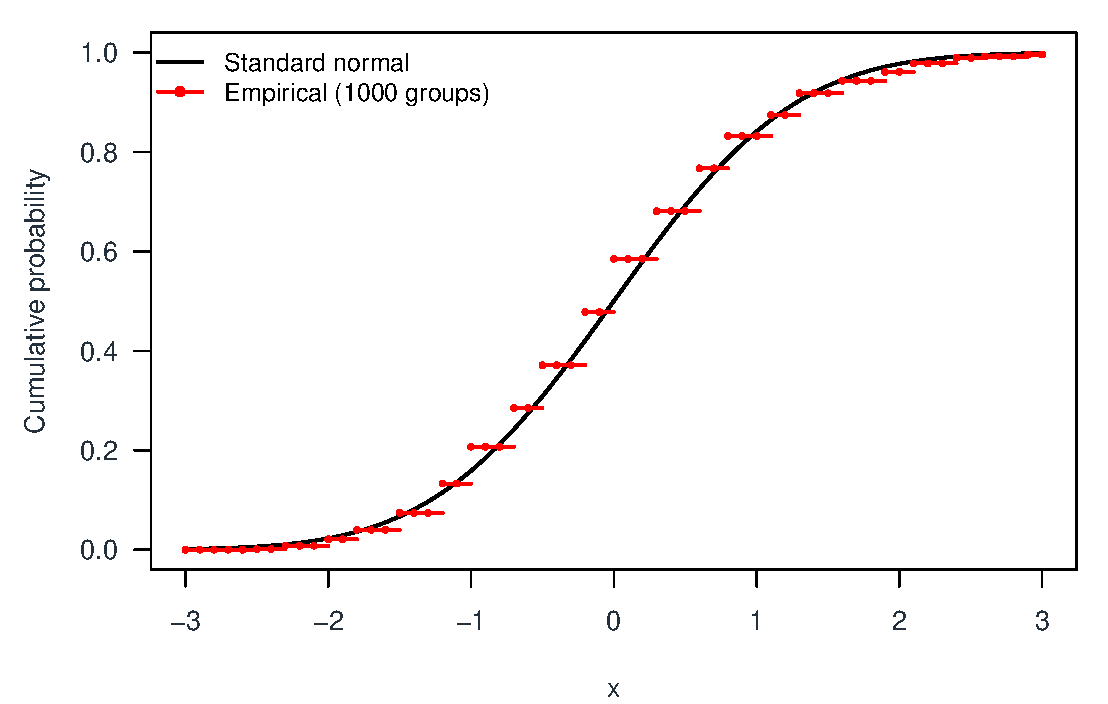
\includegraphics[width=0.96\linewidth,height=5.9cm,keepaspectratio]{poisson-n30.pdf}
  \par\smallskip
  \raggedright\small 两条曲线大体接近，但经验分布仍可见偏差与阶梯。
  \note{教材第93页图2.23。由R按例2.6.7生成1000组容量30的泊松样本，黑线Phi，红线与点是网格上的经验累计比例。第二节泊松模拟12分钟中的2分钟，教师引导读图。图只是一轮模拟，不证明定理或保证所有次数下偏差单调减小。}
\end{frame}

\begin{frame}{泊松模拟中的两个次数}
  \small
  \renewcommand{\arraystretch}{1.35}
  \begin{tabular*}{\linewidth}{@{\extracolsep{\fill}}p{0.29\linewidth}p{0.62\linewidth}@{}}
    \toprule
    \thead{数值} & \thead{含义} \\
    \midrule
    每组 $n=30$ & 每组30个观测，\newline 计算一次样本平均值。 \\
    重复1000组 & 得到1000个标准化均值，\newline 用来计算经验累计比例。 \\
    \bottomrule
  \end{tabular*}
  \par\medskip
  下一步只改变每组样本量 $n$，保持重复1000组。
  \note{教材第92--93页例2.6.7及容量改300说明。本页不另计时，包含在上一页2分钟读图内，专门区分每组样本量和组数。}
\end{frame}

\begin{frame}{课堂练习二：改变每组样本量}
  \begin{enumerate}
    \item 运行 \code{R5-class.R} 的“泊松模拟”段，\par
          观察 $n=30$ 的图形。
    \item 将 \code{n <- 30} 改为 \code{n <- 300}，\par
          重新运行该段全部代码。
    \item 保持每次1000组，比较两图中的\par
          经验分布与标准正态曲线。
    \item 说明每组样本量与重复组数\par
          分别由哪个数表示。
  \end{enumerate}
  \medskip
  使用给定程序，课堂完成，无需提交。
  \note{教材第93页例2.6.7后的n由30改为300。第二节独立练习10分钟。程序参数化后学生仅改一处，勿只重跑绘图段而未重新生成数据。}
\end{frame}

\begin{frame}[fragile]{练习二参考：需要重新计算的对象}
  \inputlabel
\begin{lstlisting}
n <- 300
y <- matrix(rpois(1000 * n, 0.5),
            1000, n)
z <- (rowSums(y) / n - 0.5) *
     sqrt(n / 0.5)
\end{lstlisting}
  随后重新运行经验累计比例与绘图代码。\par\smallskip
  此时 \code{y} 有1000行、300列，\par
  仍得到1000个标准化均值。
  \note{教材第92--93页例2.6.7。第二节讲评5分钟中的2分钟，核对n对随机数个数、矩阵列数、平均和标准化的作用，完整段只需改首行。}
\end{frame}

\begin{frame}{300个观测的样本：一次模拟结果}
  \centering
  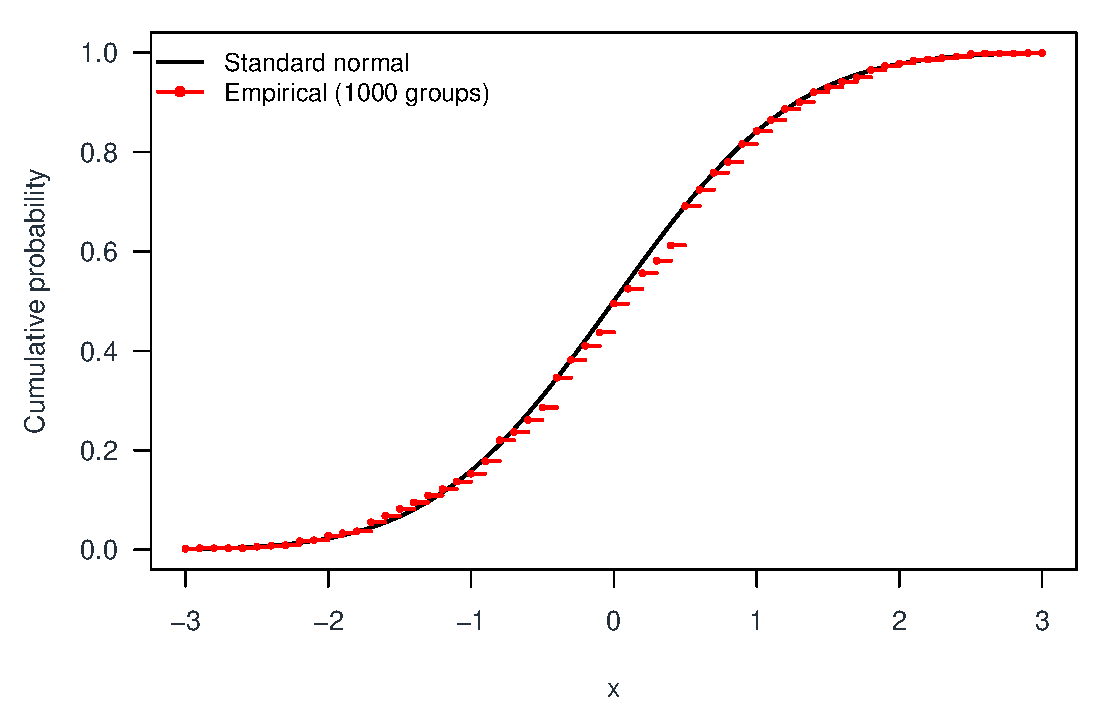
\includegraphics[width=0.96\linewidth,height=5.9cm,keepaspectratio]{poisson-n300.pdf}
  \par\smallskip
  \raggedright\small 本轮模拟的经验分布更接近标准正态曲线，仍存在随机波动。
  \note{教材第93页例2.6.7后改变样本容量的说明。图由R生成1000组容量300的泊松样本。第二节讲评5分钟中的1分钟，只比较本轮图形，不将有限次模拟视为定理证明。}
\end{frame}

\begin{frame}{本讲操作核对}
  \small
  \renewcommand{\arraystretch}{1.25}
  \begin{tabular*}{\linewidth}{@{\extracolsep{\fill}}p{0.32\linewidth}p{0.59\linewidth}@{}}
    \toprule
    \thead{任务} & \thead{本讲使用的方法} \\
    \midrule
    生成随机数 & \code{runif()}、\code{rnorm()}、\code{rpois()} \\
    估计期望与概率 & 数值平均、逻辑条件的平均 \\
    近似计算积分 & 区间长度乘函数值的平均 \\
    计算正态概率 & \code{pnorm()} 与标准化 \\
    观察正态近似 & 标准化均值的经验分布与 $\Phi$ 比较 \\
    \bottomrule
  \end{tabular*}
  \par\medskip
  模拟结果应结合概率对象与条件解释。
  \note{教材第84--93页。第二节讲评5分钟中的2分钟。第二节累计45分钟。本讲不增加误差阶、GC定理、其他积分或多维模拟，不布置提交作业。}
\end{frame}

\end{document}
